\section{TÌM KIẾM TOÀN VĂN BẢN}
\subsection{Tổng quan}
\hspace*{1cm}Tìm kiếm toàn văn bản là một phương pháp tìm kiếm thông tin trong toàn bộ nội dung của một văn bản, thay vì chỉ tìm kiếm trong tiêu đề, tóm tắt hoặc các trường chỉ mục. Điểm khác biệt giữa Tìm kiếm toàn văn bản và các kĩ thuật tìm kiếm thông thường khác là \textbf{Inverted Index}. Inverted Index là kĩ thuật tìm kiếm index theo đơn vị term thay vì index theo đơn vị row. Cụ thể hơn, Inverted Index giúp ánh xạ từ khóa tìm kiếm với các vị trí (hoặc các tài liệu) mà từ khóa đó xuất hiện. \\
Ví dụ như ở Hình \ref{fig:ftsexample}, term "new" nằm trong các document 4, 5 và 8 do đó sẽ được đánh index là 4,5,8. Việc sử dụng Inverted Index giúp cho tìm kiếm toàn văn bản trên database trở nên nhanh hơn bao giờ hết. Giả sử khi chúng ta muốn query cụm từ "Your first car", thay vì việc phải scan trên từng document một để tìm ra kết quả, bài toán tìm kiếm document chứa 3 term trên sẽ trở thành phép toán union của 3 tập hợp (document sets) của 3 term đó trong Inverted Index.\\
        \[
result = \{2,9\} \cup \{9\} \cup \{4\}
\]
\begin{figure}[H]
    \centering
    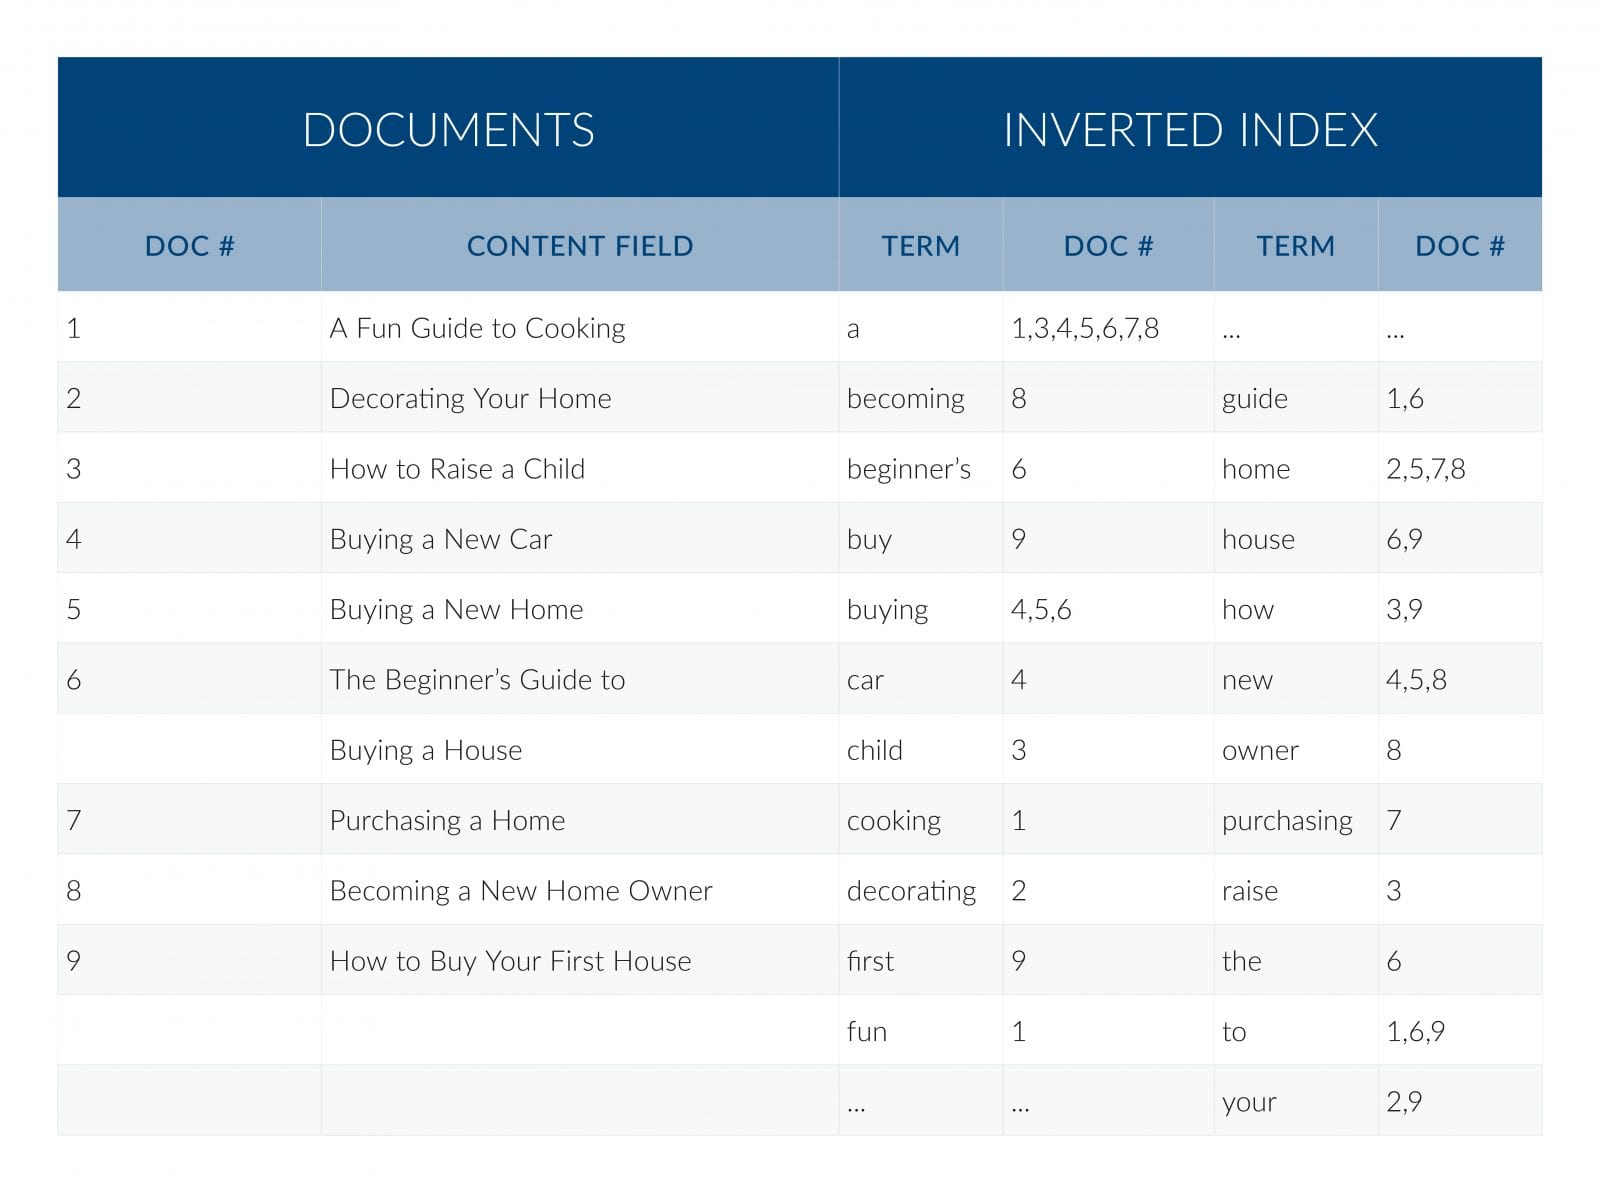
\includegraphics[width=1\textwidth]{Images/HybridSearch/FullTextSearch.png}
    \caption{Document và Term trong tìm kiếm toàn văn bản}
    \label{fig:ftsexample}
\end{figure}

\subsection{Phân tích ưu và nhược điểm}
\textbf{Ưu điểm}
\begin{itemize}
    \item \textbf{Tìm kiếm nhanh chóng và dễ dàng:} giúp tìm kiếm thông tin nhanh chóng và dễ dàng hơn, vì người dùng không cần phải biết chính xác vị trí của thông tin trong văn bản.
    \item \textbf{Có thể tìm kiếm thông tin phi cấu trúc:} có thể tìm kiếm thông tin phi cấu trúc, chẳng hạn như email, tin nhắn và tài liệu mạng xã hội.
    \item \textbf{Cải thiện trải nghiệm người dùng:} tìm kiếm thông tin hiệu quả hơn và tiết kiệm thời gian.
\end{itemize}
\textbf{Nhược điểm}
\begin{itemize}
    \item \textbf{Yêu cầu nhiều dung lượng lưu trữ:} đòi hỏi phải lưu trữ nhiều dữ liệu hơn các phương pháp tìm kiếm truyền thống, do đó nó có thể tốn kém hơn.
    \item \textbf{Kết quả có thể không chính xác hoàn toàn:} Mặc dù đã được cải tiến rất nhiều, nhưng nó vẫn có thể trả về những kết quả không chính xác hoàn toàn.
    \item \textbf{Chưa giải quyết được vấn đề từ đồng nghĩa:} Ngôn ngữ nào cũng sẽ có các từ đồng nghĩa do vậy không thể đảm bảo sẽ có thể trả về kết quả như mong muốn khi gặp phải từ đồng nghĩa
\end{itemize}